%%%% Time-stamp: <2012-08-20 17:41:39 vk>

%% example text content
%% scrartcl and scrreprt starts with section, subsection, subsubsection, ...
%% scrbook starts with part (optional), chapter, section, ...
\chapter{Background} \label{cha:background}

In this chapter, we provide preliminary information on the concepts relevant for container orchestration security.

\section{Containers}

The aim of containerisation is to simplify deployment processes and solve many of the use cases previously tackled using \acp{VM}. The main differences between containers and \acp{VM}, as explained in~\textcite{containersVsVMs}, are that when using containers, the guest OS is not virtualised on top of a hypervisor, but rather the containers run directly on the host OS using a container daemon. On the one hand, this means that the guests are not fully isolated anymore, as they are using the same host OS. This, on the other hand, however, comes with significant performance and resource benefits, which is why containers are widely replacing \acp{VM} in many use cases.

In this work, we will be primarily looking at Docker\footnote{\url{https://www.docker.com}, accessed 2019-07-18} as the container engine, yet most principles apply to any container platform.

For containerisation, the application and everything it needs is packaged into an image that is then pushed to a \textit{registry}, such as Docker Hub\footnote{\url{https://hub.docker.com}, accessed 2019-07-18}. From there, it can be pulled and executed by, for example, a container orchestration system such as Kubernetes. 

\section{Kubernetes}

\begin{figure}[H]
\begin{center}
    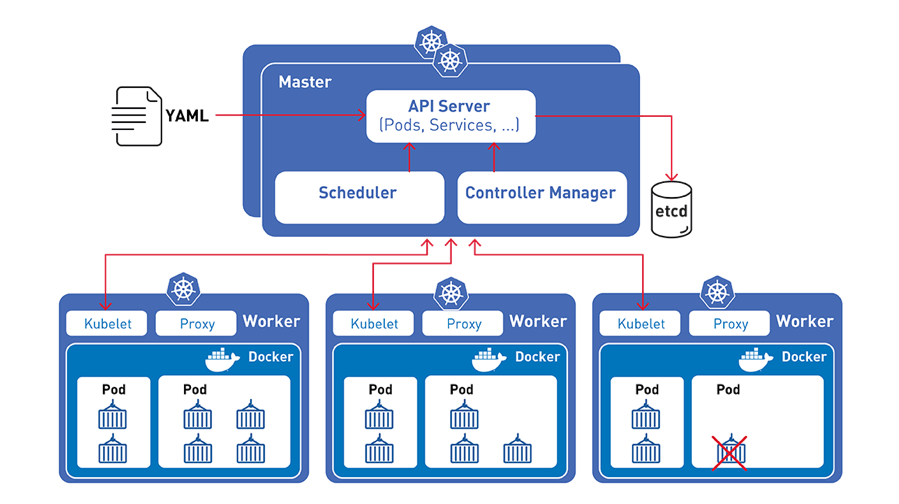
\includegraphics[width=0.8\linewidth]{figures/k8s_architecture.png}
    \caption[Kubernetes Architecture]{This architecture diagram from~\textcite{k8sDiagram} shows the typical structure of a Kubernetes cluster.}
    \label{fig:k8sArchitecture}
\end{center}
\end{figure}


Kubernetes is a highly flexible and configurable system for container orchestration that provides automating deployment, scaling, and administration of container applications, as explained in~\textcite{k8sdocs}. 

\paragraph{Architecture}

The Kubernetes architecture is depicted in Figure \ref{fig:k8sArchitecture}. It shows a \textit{cluster}, which is a set of \textit{nodes} that run the container applications. Nodes can either be physical or virtual machines. Every cluster consists of at least one master and one worker node. 

The master nodes run all so-called \textit{control-plane components} that are necessary for the cluster to function. These include the \textit{API server} and \mycode{etcd}. The \textit{API server} exposes the \textit{Kubernetes API}, which is used to control the cluster state. Administrators typically interact with the API using the CLI tool \mycode{kubectl}. \mycode{etcd} is the central key-value database that stores all cluster information and is only supposed to be accessed directly by the API server.

Worker nodes run the container daemon and the \textit{kubelet}, which is an agent responsible for managing the node. On the workers, the actual containerised applications run. The containers reside within \textit{pods}. A pod runs one or more containers on the same node. Pods are the smallest units that can be scheduled to run. They, like all other Kubernetes objects, are declaratively specified in the \textit{YAML} format. These specifications, which besides metadata and configuration information also include the URL to the registry from where the container images are pulled, are then submitted to the \textit{Kubernetes API}. The control-plane takes care of the deployment and scheduling of the specified pod. 

\paragraph{Scaling}

The power of Kubernetes lies in its more advanced concepts, including \textit{Deployments} and \textit{ReplicaSets}. These can be used to define how multiple instances of pods should be run. Kubernetes then takes care that the cluster is always in the desired state, updates are rolled out, and new replicas are spun up if required.

\paragraph{Configuration and Secrets Management}

For configuration and credentials management, Kubernetes provides the objects \textit{ConfigMap} and \textit{Secret}\footnote{\url{https://kubectl.docs.kubernetes.io/pages/app_management/secrets_and_configmaps.html}, accessed 2019-07-18}, which can be configured using YAML specifications and mounted into the containers' file systems so that applications can retrieve them.

\paragraph{Exposing applications}

To expose applications running on a set of pods, \textit{services}\footnote{\url{https://kubernetes.io/docs/concepts/services-networking/service/}, accessed 2019-07-18} can be used. They can either be employed for internal communication within the cluster or can be bound to an \textit{Ingress} to expose them to the public internet. 

%% vim:foldmethod=expr
%% vim:fde=getline(v\:lnum)=~'^%%%%\ .\\+'?'>1'\:'='
%%% Local Variables: 
%%% mode: latex
%%% mode: auto-fill
%%% mode: flyspell
%%% eval: (ispell-change-dictionary "en_US")
%%% TeX-master: "main"
%%% End: 
